\documentclass{article}
\usepackage[utf8]{inputenc}
\usepackage{enumerate}
\usepackage{enumitem}
\usepackage{float}
\usepackage{graphicx}
\usepackage{multirow, array}


\title{Práctica 2: Gestión de una Web de cine}
\author{Rafael Nogales Vaquero
\\Lothar Soto Palma
\\Elena Toro Pérez
\\Jose Ramón Trillo Vilchez}
\date{5 Noviembre del 2014}

\begin{document}

\maketitle

\section{Introducción}
\section{Jerarquia de casos de uso}
\subsection*{Gestión de Usuarios}
	\begin{description}
	\item[Descripción]:\\ Escenarios asociados con la gestión de usuarios,clientes y administradores/empleados.
	\item[Casos de Uso]:\\ Registro(Alta usuario), Consultar películas, Modificar información de usuario, Consultar información de Usuario, Consultar cuenta de Usuario, Votar Películas, Comentar/criticar Películas, Eliminar cuenta de Usuario, Acceder a lista de Almas Gemelas, Comprar Película, Comprar Película, Consulta a Empleado/Administrador, Identificar Usuario, Método de pago, Actualizar Películas, Añadir/borrar Películas, Control de comentarios/críticas, Moderación de usuarios, Listar usuarios Baneados del sistema, Listar usuarios colaboradores, Banear usuarios.
	\item[Actores]:\\ Cliente, Usuario, Administrador, Sistema.
	\end{description}
\subsection*{Gestión de Almas Gemelas}
\subsection*{Gestión de Películas}
\subsection*{Gestión de Ventas}
	\begin{description}
	\item[Descripción]:\\ Escenarios asociados con la gestión de ventas de películas.
	\item[Casos de Uso]:\\ Comprar Película, Reservar Película, Identificar Socio, Disponibilidad de Películas, Pago a Cuenta, Pago en Metálico, Pago con Tarjeta.
	\item[Actores]:\\ Usuario, Administrador.
	\end{description}
\section{Diagrama de paquetes}
	\begin{figure}[h]
		\begin{center}
   			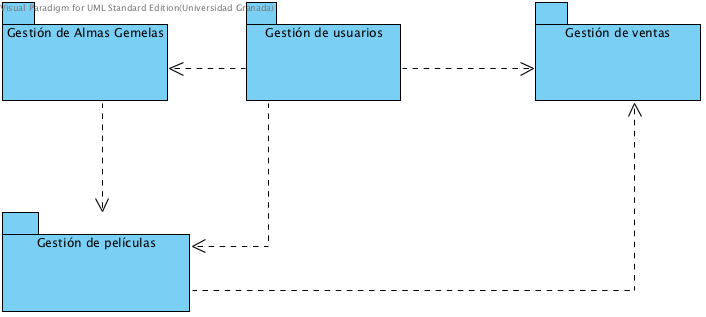
\includegraphics[scale=0.75]{Paquetes.png}
 	  	\end{center}
 	 \end{figure}


\section{Diagrama de casos de uso}
\subsection*{Gestión de Usuarios}
		\begin{center}
   			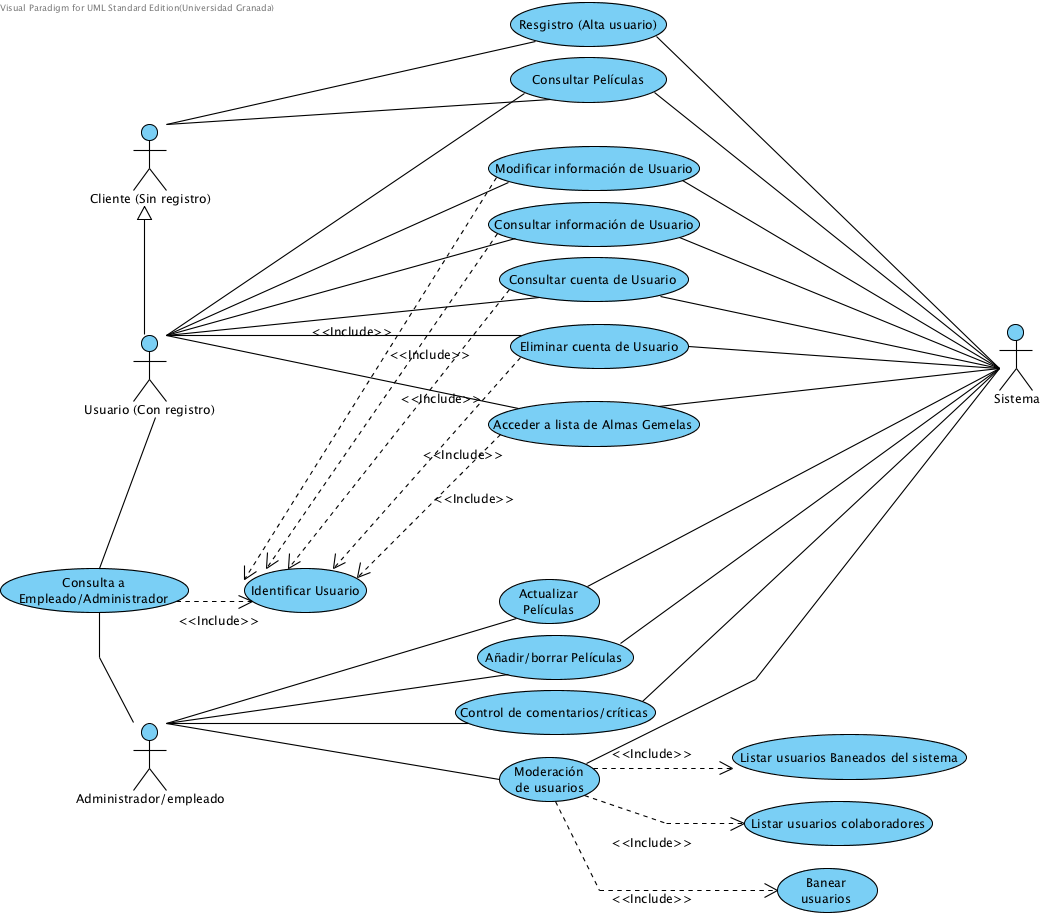
\includegraphics[scale=0.65]{GestiondeUsuarios.png}
   		\end{center}	

\section{Descripción básica de casos de uso}
\begin{table}[h]
\begin{tabular}{|l|l|l|l|l|l|}
\hline
\multicolumn{2}{|p{2cm}|}{Casos de uso}  & \multicolumn{3}{p{7cm}|}{Registro(Alta usuario)} & CU-x \\
\hline
\multicolumn{2}{|p{2cm}|}{Actores}       & \multicolumn{4}{p{8cm}|}{Cliente (Sin registro), Sistema}        \\
\hline
\multicolumn{2}{|p{2cm}|}{Tipo}          & \multicolumn{4}{p{8cm}|}{Primario, Esencial}        \\
\hline
\multicolumn{2}{|p{2cm}|}{Precondición}  & \multicolumn{4}{p{8cm}|}{El cliente no debe poseer cuenta y por tanto no tiene un registro en el sistema.}        \\
\hline
\multicolumn{2}{|p{2cm}|}{Postcondición} & \multicolumn{4}{p{8cm}|}{}        \\
\hline
\multicolumn{6}{|p{10cm}|}{Proposito}                                   \\
\hline
\multicolumn{6}{|p{10cm}|}{Registrar a los clientes sin cuenta en el sistema.}                                            \\
\hline
\multicolumn{6}{|p{10cm}|}{Descripción}                                 \\
\hline
\multicolumn{6}{|p{10cm}|}{El cliente se registra en el sistema para acceder a las opciones del sistema de la que solo pueden hacer uso los usuarios(con registro).}                                            \\
\hline
Autor              &     Lothar Soto         & Fecha    &  8/11/04   &   Versión  & 1\\     
\hline
\end{tabular}
\end{table}
\begin{table}[h]
\begin{tabular}{|l|l|l|l|l|l|}
\hline
\multicolumn{2}{|p{2cm}|}{Casos de uso}  & \multicolumn{3}{p{7cm}|}{Consultar Películas} & CU-x \\
\hline
\multicolumn{2}{|p{2cm}|}{Actores}       & \multicolumn{4}{p{8cm}|}{Cliente (Sin registro),Usuario(Con registro) , Sistema}        \\
\hline
\multicolumn{2}{|p{2cm}|}{Tipo}          & \multicolumn{4}{p{8cm}|}{Primario, Esencial}        \\
\hline
\multicolumn{2}{|p{2cm}|}{Precondición}  & \multicolumn{4}{p{8cm}|}{}        \\
\hline
\multicolumn{2}{|p{2cm}|}{Postcondición} & \multicolumn{4}{p{8cm}|}{}        \\
\hline
\multicolumn{6}{|p{10cm}|}{Proposito}                                   \\
\hline
\multicolumn{6}{|p{10cm}|}{Que se pueda acceder a información y multimedia hacerca de una película.}                                            \\
\hline
\multicolumn{6}{|p{10cm}|}{Descripción}                                 \\
\hline
\multicolumn{6}{|p{10cm}|}{Permite a los clientes, usuarios acceder a informcación acerca de la película buscada.}                                            \\
\hline
Autor              &     Lothar Soto         & Fecha    &  8/11/04   &   Versión  & 1\\     
\hline
\end{tabular}
\end{table}
\begin{table}[h]
\begin{tabular}{|l|l|l|l|l|l|}
\hline
\multicolumn{2}{|p{2cm}|}{Casos de uso}  & \multicolumn{3}{p{7cm}|}{Modificar información de Usuario} & CU-x \\
\hline
\multicolumn{2}{|p{2cm}|}{Actores}       & \multicolumn{4}{p{8cm}|}{Usuario (Con registro), Sistema}        \\
\hline
\multicolumn{2}{|p{2cm}|}{Tipo}          & \multicolumn{4}{p{8cm}|}{Primario, Esencial}        \\
\hline
\multicolumn{2}{|p{2cm}|}{Precondición}  & \multicolumn{4}{p{8cm}|}{Debe ser un Usuario por lo que se tiene que estar registrado previamente.}        \\
\hline
\multicolumn{2}{|p{2cm}|}{Postcondición} & \multicolumn{4}{p{8cm}|}{}        \\
\hline
\multicolumn{6}{|p{10cm}|}{Proposito}                                   \\
\hline
\multicolumn{6}{|p{10cm}|}{Conseguir la comodidad con los datos del usuario y que este puede modificarlos dentro de ciertas limitaciones.}                                            \\
\hline
\multicolumn{6}{|p{10cm}|}{Descripción}                                 \\
\hline
\multicolumn{6}{|p{10cm}|}{El usuario modifica su información de cuenta como el Correo, Contraseaña...}                                            \\
\hline
Autor              &     Lothar Soto         & Fecha    &  8/11/04   &   Versión  & 1.0\\     
\hline
\end{tabular}
\end{table}
\begin{table}[h]
\begin{tabular}{|l|l|l|l|l|l|}
\hline
\multicolumn{2}{|p{2cm}|}{Casos de uso}  & \multicolumn{3}{p{7cm}|}{Consultar información de Usuario} & CU-x \\
\hline
\multicolumn{2}{|p{2cm}|}{Actores}       & \multicolumn{4}{p{8cm}|}{Usuario (Con registro), Sistema}        \\
\hline
\multicolumn{2}{|p{2cm}|}{Tipo}          & \multicolumn{4}{p{8cm}|}{Primario, Esencial}        \\
\hline
\multicolumn{2}{|p{2cm}|}{Precondición}  & \multicolumn{4}{p{8cm}|}{Debe ser un Usuario por lo que se tiene que estar registrado previamente.}        \\
\hline
\multicolumn{2}{|p{2cm}|}{Postcondición} & \multicolumn{4}{p{8cm}|}{}        \\
\hline
\multicolumn{6}{|p{10cm}|}{Proposito}                                   \\
\hline
\multicolumn{6}{|p{10cm}|}{Conseguir la comodidad con los datos del usuario y que este pueda consultarlos en cualquier momento.}                                            \\
\hline
\multicolumn{6}{|p{10cm}|}{Descripción}                                 \\
\hline
\multicolumn{6}{|p{10cm}|}{El usuario consulta su información de cuenta como el estado,gustos...}                                            \\
\hline
Autor              &     Lothar Soto         & Fecha    &  8/11/04   &   Versión  & 1.0\\     
\hline
\end{tabular}
\end{table}
\begin{table}[h]
\begin{tabular}{|l|l|l|l|l|l|}
\hline
\multicolumn{2}{|p{2cm}|}{Casos de uso}  & \multicolumn{3}{p{7cm}|}{Consultar cuenta de Usuario} & CU-x \\
\hline
\multicolumn{2}{|p{2cm}|}{Actores}       & \multicolumn{4}{p{8cm}|}{Usuario (Con registro), Sistema}        \\
\hline
\multicolumn{2}{|p{2cm}|}{Tipo}          & \multicolumn{4}{p{8cm}|}{Primario, Esencial}        \\
\hline
\multicolumn{2}{|p{2cm}|}{Precondición}  & \multicolumn{4}{p{8cm}|}{Se debe poseer una cuenta de usuario (registrado).}        \\
\hline
\multicolumn{2}{|p{2cm}|}{Postcondición} & \multicolumn{4}{p{8cm}|}{}        \\
\hline
\multicolumn{6}{|p{10cm}|}{Proposito}                                   \\
\hline
\multicolumn{6}{|p{10cm}|}{Poder consultar su información agregada en el momento del registro.}                                            \\
\hline
\multicolumn{6}{|p{10cm}|}{Descripción}                                 \\
\hline
\multicolumn{6}{|p{10cm}|}{Permite a los usuarios consultar sus datos de cuenta en caso de olvido como el Correo, o contraseña(Este último requiere confirmación).}                                            \\
\hline
Autor             &     Lothar Soto          & Fecha    &  8/11/04   &   Versión  &1.0\\     
\hline
\end{tabular}
\end{table}
\begin{table}[h]
\begin{tabular}{|l|l|l|l|l|l|}
\hline
\multicolumn{2}{|p{2cm}|}{Casos de uso}  & \multicolumn{3}{p{7cm}|}{Votar Películas} & CU-x \\
\hline
\multicolumn{2}{|p{2cm}|}{Actores}       & \multicolumn{4}{p{8cm}|}{Usuario(Con registro), Sistema}        \\
\hline
\multicolumn{2}{|p{2cm}|}{Tipo}          & \multicolumn{4}{p{8cm}|}{Primario, Esencial}        \\
\hline
\multicolumn{2}{|p{2cm}|}{Precondición}  & \multicolumn{4}{p{8cm}|}{Se debe poseer una cuenta de usuario (registrado).}        \\
\hline
\multicolumn{2}{|p{2cm}|}{Postcondición} & \multicolumn{4}{p{8cm}|}{}        \\
\hline
\multicolumn{6}{|p{10cm}|}{Proposito}                                   \\
\hline
\multicolumn{6}{|p{10cm}|}{Dar la opinión de los usuarios sobre las películas a modo de voto.}                                            \\
\hline
\multicolumn{6}{|p{10cm}|}{Descripción}                                 \\
\hline
\multicolumn{6}{|p{10cm}|}{Permite al usuario votar una película positiva o negativamente.}                                            \\
\hline
Autor          &       Lothar Soto        & Fecha    &  8/11/04   &   Versión  & 1.0\\     
\hline
\end{tabular}
\end{table}
\begin{table}[h]
\begin{tabular}{|l|l|l|l|l|l|}
\hline
\multicolumn{2}{|p{2cm}|}{Casos de uso}  & \multicolumn{3}{p{7cm}|}{Eliminar cuenta de Usuario} & CU-x \\
\hline
\multicolumn{2}{|p{2cm}|}{Actores}       & \multicolumn{4}{p{8cm}|}{Usuario(Con registro), Sistema}        \\
\hline
\multicolumn{2}{|p{2cm}|}{Tipo}          & \multicolumn{4}{p{8cm}|}{Primario, Esencial}        \\
\hline
\multicolumn{2}{|p{2cm}|}{Precondición}  & \multicolumn{4}{p{8cm}|}{Se debe poseer una cuenta de usuario (registrado).}        \\
\hline
\multicolumn{2}{|p{2cm}|}{Postcondición} & \multicolumn{4}{p{8cm}|}{}        \\
\hline
\multicolumn{6}{|p{10cm}|}{Proposito}                                   \\
\hline
\multicolumn{6}{|p{10cm}|}{Dar de baja a un usuario y posteriormente eliminar su cuenta.}                                            \\
\hline
\multicolumn{6}{|p{10cm}|}{Descripción}                                 \\
\hline
\multicolumn{6}{|p{10cm}|}{Permite al usuario dejar de usar el sistema sin que quede información de este en el mismo.}                                            \\
\hline
Autor          &       Lothar Soto        & Fecha    &  8/11/04   &   Versión  & 1.0\\     
\hline
\end{tabular}
\end{table}
\begin{table}[h]
\begin{tabular}{|l|l|l|l|l|l|}
\hline
\multicolumn{2}{|p{2cm}|}{Casos de uso}  & \multicolumn{3}{p{7cm}|}{Acceder a lista de almas gemelas} & CU-x \\
\hline
\multicolumn{2}{|p{2cm}|}{Actores}       & \multicolumn{4}{p{8cm}|}{Usuario(Con registro), Sistema}        \\
\hline
\multicolumn{2}{|p{2cm}|}{Tipo}          & \multicolumn{4}{p{8cm}|}{Primario, Esencial}        \\
\hline
\multicolumn{2}{|p{2cm}|}{Precondición}  & \multicolumn{4}{p{8cm}|}{Se debe poseer una cuenta de usuario (registrado).}        \\
\hline
\multicolumn{2}{|p{2cm}|}{Postcondición} & \multicolumn{4}{p{8cm}|}{}        \\
\hline
\multicolumn{6}{|p{10cm}|}{Proposito}                                   \\
\hline
\multicolumn{6}{|p{10cm}|}{Dar a conocer al usuario una serie de personas que tienen los mismos gustos que dicha persona.}                                            \\
\hline
\multicolumn{6}{|p{10cm}|}{Descripción}                                 \\
\hline
\multicolumn{6}{|p{10cm}|}{Permite dar al usuario conocimiento de que personas comparten sus gustos y en parte están relacionadas con él.}                                            \\
\hline
Autor          &       Lothar Soto        & Fecha    &  8/11/04   &   Versión  & 1.0\\    
\hline
\end{tabular}
\end{table}

\begin{table}[h]
\begin{tabular}{|l|l|l|l|l|l|}
\hline
\multicolumn{2}{|p{2cm}|}{Casos de uso}  & \multicolumn{3}{p{7cm}|}{Identificar Usuario} & CU-x \\
\hline
\multicolumn{2}{|p{2cm}|}{Actores}       & \multicolumn{4}{p{8cm}|}{Usuario (Con registro), Sistema}        \\
\hline
\multicolumn{2}{|p{2cm}|}{Tipo}          & \multicolumn{4}{p{8cm}|}{Secundario, Esencial}        \\
\hline
\multicolumn{2}{|p{2cm}|}{Precondición}  & \multicolumn{4}{p{8cm}|}{Se debe poseer una cuenta de usuario (registrado).}        \\
\hline
\multicolumn{2}{|p{2cm}|}{Postcondición} & \multicolumn{4}{p{8cm}|}{}        \\
\hline
\multicolumn{6}{|p{10cm}|}{Proposito}                                   \\
\hline
\multicolumn{6}{|p{10cm}|}{Proporcionar una identidad a un usuario en el sistema.}                                            \\
\hline
\multicolumn{6}{|p{10cm}|}{Descripción}                                 \\
\hline
\multicolumn{6}{|p{10cm}|}{Permite a los usuarios identificarse en el sistema para posteriormente realizar distintas operaciones.}                                            \\
\hline
Autor          &       Lothar Soto        & Fecha    &  8/11/04   &   Versión  & 1.0\\    
\hline
\end{tabular}
\end{table}

\begin{table}[h]
\begin{tabular}{|l|l|l|l|l|l|}
\hline
\multicolumn{2}{|p{2cm}|}{Casos de uso}  & \multicolumn{3}{p{7cm}|}{Consulta a Empleado/Administrador} & CU-x \\
\hline
\multicolumn{2}{|p{2cm}|}{Actores}       & \multicolumn{4}{p{8cm}|}{Usuario (Con registro), Administrador/Empleado}        \\
\hline
\multicolumn{2}{|p{2cm}|}{Tipo}          & \multicolumn{4}{p{8cm}|}{Primario, Esencial}        \\
\hline
\multicolumn{2}{|p{2cm}|}{Precondición}  & \multicolumn{4}{p{8cm}|}{Se debe poseer una cuenta de usuario (registrado).}        \\
\hline
\multicolumn{2}{|p{2cm}|}{Postcondición} & \multicolumn{4}{p{8cm}|}{}        \\
\hline
\multicolumn{6}{|p{10cm}|}{Proposito}                                   \\
\hline
\multicolumn{6}{|p{10cm}|}{Contactar el usuario con un administrador o empleado.}                                            \\
\hline
\multicolumn{6}{|p{10cm}|}{Descripción}                                 \\
\hline
\multicolumn{6}{|p{10cm}|}{El usuario podrá usar esta funcionalidad para contactar con un administrador para resolver algún tipo de incidencia o duda.}                                            \\
\hline
Autor          &       Lothar Soto        & Fecha    &  8/11/04   &   Versión  & 1.0\\    
\hline
\end{tabular}
\end{table}

\begin{table}[h]
\begin{tabular}{|l|l|l|l|l|l|}
\hline
\multicolumn{2}{|p{2cm}|}{Casos de uso}  & \multicolumn{3}{p{7cm}|}{Actualizar Películas} & CU-x \\
\hline
\multicolumn{2}{|p{2cm}|}{Actores}       & \multicolumn{4}{p{8cm}|}{Administrador/Empleado, Sistema}        \\
\hline
\multicolumn{2}{|p{2cm}|}{Tipo}          & \multicolumn{4}{p{8cm}|}{Primario, Esencial}        \\
\hline
\multicolumn{2}{|p{2cm}|}{Precondición}  & \multicolumn{4}{p{8cm}|}{Necesario tener los permisos de administrador o empleado del sistema.}        \\
\hline
\multicolumn{2}{|p{2cm}|}{Postcondición} & \multicolumn{4}{p{8cm}|}{}        \\
\hline
\multicolumn{6}{|p{10cm}|}{Proposito}                                   \\
\hline
\multicolumn{6}{|p{10cm}|}{Actualizar la lista de películas disponibles.}                                            \\
\hline
\multicolumn{6}{|p{10cm}|}{Descripción}                                 \\
\hline
\multicolumn{6}{|p{10cm}|}{Permite actualizar la lista de películas si anteriormente se ha añadido una o borrado.}                                            \\
\hline
Autor          &       Lothar Soto        & Fecha    &  8/11/04   &   Versión  & 1.0\\    
\hline
\end{tabular}
\end{table}

\begin{table}[h]
\begin{tabular}{|l|l|l|l|l|l|}
\hline
\multicolumn{2}{|p{2cm}|}{Casos de uso}  & \multicolumn{3}{p{7cm}|}{Añadir/Borrar Películas} & CU-x \\
\hline
\multicolumn{2}{|p{2cm}|}{Actores}       & \multicolumn{4}{p{8cm}|}{Administrador/Empleado, Sistema}        \\
\hline
\multicolumn{2}{|p{2cm}|}{Tipo}          & \multicolumn{4}{p{8cm}|}{Primario, Esencial}        \\
\hline
\multicolumn{2}{|p{2cm}|}{Precondición}  & \multicolumn{4}{p{8cm}|}{Necesario tener los permisos de administrador o empleado del sistema.}        \\
\hline
\multicolumn{2}{|p{2cm}|}{Postcondición} & \multicolumn{4}{p{8cm}|}{}        \\
\hline
\multicolumn{6}{|p{10cm}|}{Proposito}                                   \\
\hline
\multicolumn{6}{|p{10cm}|}{Conseguir una lista actualizada de películas en el sistema.}                                            \\
\hline
\multicolumn{6}{|p{10cm}|}{Descripción}                                 \\
\hline
\multicolumn{6}{|p{10cm}|}{Permite a los empleados y administradores añadir películas al sistema y borrarlas dependiende de lo que interese.}                                            \\
\hline
Autor          &       Lothar Soto        & Fecha    &  8/11/04   &   Versión  & 1.0\\    
\hline
\end{tabular}
\end{table}

\begin{table}[h]
\begin{tabular}{|l|l|l|l|l|l|}
\hline
\multicolumn{2}{|p{2cm}|}{Casos de uso}  & \multicolumn{3}{p{7cm}|}{Control de comentarios/críticas} & CU-x \\
\hline
\multicolumn{2}{|p{2cm}|}{Actores}       & \multicolumn{4}{p{8cm}|}{Administrador/Empleado, Sistema}        \\
\hline
\multicolumn{2}{|p{2cm}|}{Tipo}          & \multicolumn{4}{p{8cm}|}{Primario, Esencial}        \\
\hline
\multicolumn{2}{|p{2cm}|}{Precondición}  & \multicolumn{4}{p{8cm}|}{Necesario tener los permisos de administrador o empleado del sistema.}        \\
\hline
\multicolumn{2}{|p{2cm}|}{Postcondición} & \multicolumn{4}{p{8cm}|}{}        \\
\hline
\multicolumn{6}{|p{10cm}|}{Proposito}                                   \\
\hline
\multicolumn{6}{|p{10cm}|}{Controlar los comentarios de los usuarios puesto pueden resultar inapropiados.}                                            \\
\hline
\multicolumn{6}{|p{10cm}|}{Descripción}                                 \\
\hline
\multicolumn{6}{|p{10cm}|}{Permite a los empleados y administradores  manejar los comentarios (pueden eliminarlos).}                                            \\
\hline
Autor          &       Lothar Soto        & Fecha    &  8/11/04   &   Versión  & 1.0\\    
\hline
\end{tabular}
\end{table}
\begin{table}[h]
\begin{tabular}{|l|l|l|l|l|l|}
\hline
\multicolumn{2}{|p{2cm}|}{Casos de uso}  & \multicolumn{3}{p{7cm}|}{Moderación de Usuarios} & CU-x \\
\hline
\multicolumn{2}{|p{2cm}|}{Actores}       & \multicolumn{4}{p{8cm}|}{Administrador/Empleado, Sistema}        \\
\hline
\multicolumn{2}{|p{2cm}|}{Tipo}          & \multicolumn{4}{p{8cm}|}{Primario, Esencial}        \\
\hline
\multicolumn{2}{|p{2cm}|}{Precondición}  & \multicolumn{4}{p{8cm}|}{Necesario tener los permisos de administrador o empleado del sistema.}        \\
\hline
\multicolumn{2}{|p{2cm}|}{Postcondición} & \multicolumn{4}{p{8cm}|}{}        \\
\hline
\multicolumn{6}{|p{10cm}|}{Proposito}                                   \\
\hline
\multicolumn{6}{|p{10cm}|}{Controlar el comportamiento de los usuarios en el sistema.}                                            \\
\hline
\multicolumn{6}{|p{10cm}|}{Descripción}                                 \\
\hline
\multicolumn{6}{|p{10cm}|}{Permite a los empleados y administradores controlar a los usuarios usando un métodos de sanciones.}                                            \\
\hline
Autor          &       Lothar Soto        & Fecha    &  8/11/04   &   Versión  & 1.0\\    
\hline
\end{tabular}
\end{table}

\begin{table}[h]
\begin{tabular}{|l|l|l|l|l|l|}
\hline
\multicolumn{2}{|p{2cm}|}{Casos de uso}  & \multicolumn{3}{p{7cm}|}{Listar usuarios Baneados del sistema} & CU-x \\
\hline
\multicolumn{2}{|p{2cm}|}{Actores}       & \multicolumn{4}{p{8cm}|}{Administrador/Empleado, Sistema}        \\
\hline
\multicolumn{2}{|p{2cm}|}{Tipo}          & \multicolumn{4}{p{8cm}|}{Secundario, Esencial}        \\
\hline
\multicolumn{2}{|p{2cm}|}{Precondición}  & \multicolumn{4}{p{8cm}|}{Necesario tener los permisos de administrador o empleado del sistema.}        \\
\hline
\multicolumn{2}{|p{2cm}|}{Postcondición} & \multicolumn{4}{p{8cm}|}{}        \\
\hline
\multicolumn{6}{|p{10cm}|}{Proposito}                                   \\
\hline
\multicolumn{6}{|p{10cm}|}{Obtener una lista de los usuarios baneados del sistema.}                                            \\
\hline
\multicolumn{6}{|p{10cm}|}{Descripción}                                 \\
\hline
\multicolumn{6}{|p{10cm}|}{Permite al administrador conocer los usuarios baneados.}                                            \\
\hline
Autor          &       Lothar Soto        & Fecha    &  8/11/04   &   Versión  & 1.0\\    
\hline
\end{tabular}
\end{table}

\begin{table}[h]
\begin{tabular}{|l|l|l|l|l|l|}
\hline
\multicolumn{2}{|p{2cm}|}{Casos de uso}  & \multicolumn{3}{p{7cm}|}{Listar Usuarios Colaboradores} & CU-x \\
\hline
\multicolumn{2}{|p{2cm}|}{Actores}       & \multicolumn{4}{p{8cm}|}{Administrador/Empleado, Sistema}        \\
\hline
\multicolumn{2}{|p{2cm}|}{Tipo}          & \multicolumn{4}{p{8cm}|}{Secundario, Esencial}        \\
\hline
\multicolumn{2}{|p{2cm}|}{Precondición}  & \multicolumn{4}{p{8cm}|}{Necesario tener los permisos de administrador o empleado del sistema.}        \\
\hline
\multicolumn{2}{|p{2cm}|}{Postcondición} & \multicolumn{4}{p{8cm}|}{}        \\
\hline
\multicolumn{6}{|p{10cm}|}{Proposito}                                   \\
\hline
\multicolumn{6}{|p{10cm}|}{Obtener una liste de los usuarios que colaboraron en el sistema.}                                            \\
\hline
\multicolumn{6}{|p{10cm}|}{Descripción}                                 \\
\hline
\multicolumn{6}{|p{10cm}|}{Permite al administrador conocer a los usuarios colaboradores.}                                            \\
\hline
Autor          &       Lothar Soto        & Fecha    &  8/11/04   &   Versión  & 1.0\\    
\hline
\end{tabular}
\end{table}

\begin{table}[h]
\begin{tabular}{|l|l|l|l|l|l|}
\hline
\multicolumn{2}{|p{2cm}|}{Casos de uso}  & \multicolumn{3}{p{7cm}|}{Banear Usuario} & CU-x \\
\hline
\multicolumn{2}{|p{2cm}|}{Actores}       & \multicolumn{4}{p{8cm}|}{Administrador/Empleado, Sistema}        \\
\hline
\multicolumn{2}{|p{2cm}|}{Tipo}          & \multicolumn{4}{p{8cm}|}{Secundario, Esencial}        \\
\hline
\multicolumn{2}{|p{2cm}|}{Precondición}  & \multicolumn{4}{p{8cm}|}{Necesario tener los permisos de administrador o empleado del sistema.}        \\
\hline
\multicolumn{2}{|p{2cm}|}{Postcondición} & \multicolumn{4}{p{8cm}|}{}        \\
\hline
\multicolumn{6}{|p{10cm}|}{Proposito}                                   \\
\hline
\multicolumn{6}{|p{10cm}|}{Denegar el acceso a un usuario conflictivo.}                                            \\
\hline
\multicolumn{6}{|p{10cm}|}{Descripción}                                 \\
\hline
\multicolumn{6}{|p{10cm}|}{Permite a los administradores y empleados denegar el acceso a un usuario conflictivo del sistema.}                                            \\
\hline
Autor          &       Lothar Soto        & Fecha    &  8/11/04   &   Versión  & 1.0\\    
\hline
\end{tabular}
\end{table}



%======================================
%Ejemplo de tabla de casos de uso:
%======================================
\begin{table}[h]
\begin{tabular}{|l|l|l|l|l|l|}
\hline
\multicolumn{2}{|p{2cm}|}{Casos de uso}  & \multicolumn{3}{p{7cm}|}{} & CU-x \\
\hline
\multicolumn{2}{|p{2cm}|}{Actores}       & \multicolumn{4}{p{8cm}|}{}        \\
\hline
\multicolumn{2}{|p{2cm}|}{Tipo}          & \multicolumn{4}{p{8cm}|}{}        \\
\hline
\multicolumn{2}{|p{2cm}|}{Precondición}  & \multicolumn{4}{p{8cm}|}{}        \\
\hline
\multicolumn{2}{|p{2cm}|}{Postcondición} & \multicolumn{4}{p{8cm}|}{}        \\
\hline
\multicolumn{6}{|p{10cm}|}{Proposito}                                   \\
\hline
\multicolumn{6}{|p{10cm}|}{}                                            \\
\hline
\multicolumn{6}{|p{10cm}|}{Descripción}                                 \\
\hline
\multicolumn{6}{|p{10cm}|}{}                                            \\
\hline
Autor              &              & Fecha    &     &   Versión  &\\     
\hline
\end{tabular}
\end{table}


\end{document}
